\chapter{基于深度卷积网络的线虫轮廓解析}
	多线虫跟踪问题中,多线虫轮廓之间相互遮挡是造成线虫跟踪丢失的主要原因,是实现线虫长期跟踪的关键。
	如图\ref{fig:multiworm}所示,是一张经过前景轮廓提取后得到的一幅二值化图片,图中线虫轮廓之间出现严重的相互遮挡的情况
	。虽然人眼可以很轻松的辨别出图中所有单个线虫的轮廓,但自动化地线虫轮廓解析却十分困难,尽管深度学习在图像分割任务中取得了很大的成功,
	但线虫轮廓的解析不同于图像分割,因此不能直接转为一个端到端的学习问题。
	本文提出了一种基于深度卷积网络的线虫轮廓解析的方法尝试解决这一问题,并探讨了多种网络结构的设计对识别性能的影响。
	\begin{figure}[h]
	  \centering
	  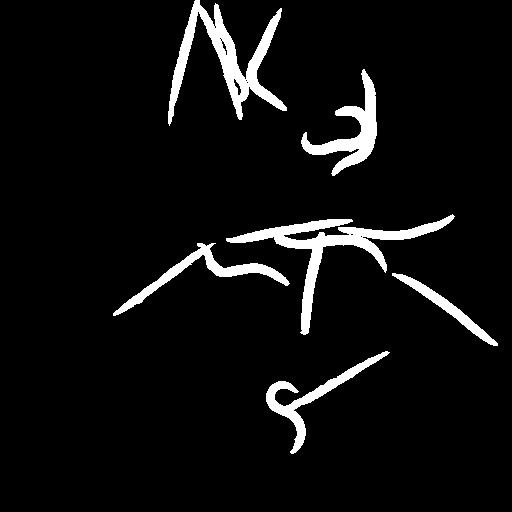
\includegraphics[width=7cm]{figure/chap4/multi-worm.jpg}
	  \bicaption[这里将出现在插图索引中]
		{多线虫轮廓相互遮挡图片}
		{Change in contour curvature}
	  \label{fig:multiworm}
	\end{figure}
\section{卷积神经网络介绍}
	从1956年正式提出人工智能学科以来,人工智能领域的研究经历了60年的发展。期间,不同学科背景的学者们对人工智能的实现,提出
	了不同的观点并由此产生了不同的学术流派。其中对人工智能领域影响较大的主要有符号主义(Symbolism)、
	连接主义(Connectionism)和进化主义(Evolutionism)或控制论学派(Cyberneticsism)等。
	目前,在诸多领域取得重大突破的深度学习(Deep learning)技术是连接主义学派的典型代表性技术。其主要受
	神经科学的启发,大脑中大量的神经元形成复杂的连接,信号在神经元之间传递。人工神经网络(Artificial Neural Network,ANN)
	利用大量相互连接的节点构成,每个节点代表一个特定激活函数的输出,两个节点之间的连接都有一个权重。通常,神经网络模型
	都是由多层网络堆叠而成,前一层网络的输出作为后一层网络的输入。从网络的输出来看,整个网络的输出相当于由许多张量函数嵌套构成的
	复合函数,网络模型参数的训练依赖的误差反向传播的算法其实质是复合函数的链式求导法则。
	
	卷积网络(Cnvolutional Neural Network,CNN)是人工神经网络模型中的一种,由Yan Lecun于1989年提出并将其用于手写数字识别
	\cite{le1989handwritten},卷积操作类似于图像处理中的空间滤波,不同的是滤波核作为模型参数是通过学习得到的。
	一个典型的卷积网络架构如图\ref{fig:chap4:cnn}所示,通常由卷积层,池化层,全连接层等构成。为了使模型具有更好的泛化
	性能,通常在不同的层之间还会加入Dropout层和Batch Normalization层。自2006年以来,研究者们不断对卷积网络进行改进提出
	了很多性能优异的网络架构(如:AlexNet网络\cite{krizhevsky2012imagenet}、VGG网络\cite{simonyan2014very}、
	GoogLenet网络\cite{szegedy2015going}和ResNet网络\cite{Kaiming2015Deep})。使卷积网络在许多计算机视觉任务中大放异彩。
	\begin{figure}[h]
	  \centering
	  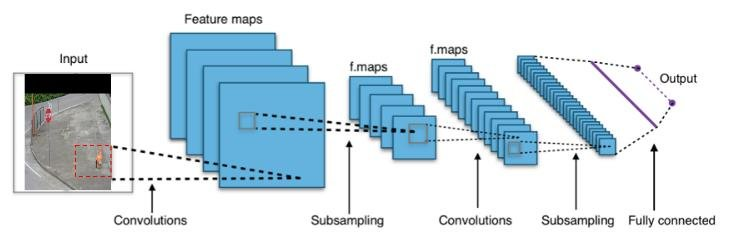
\includegraphics[width=12cm]{figure/chap4/CNN-arch.png}
	  \bicaption[这里将出现在插图索引中]
		{卷积网络的经典结构}
		{A typical architecture of CNN}
	  \label{fig:chap4:cnn}
	\end{figure}
\subsection{卷积层}
	卷积层是卷积网络中主要的连接层,由于其引入权值共享的机制,与全连接的方式相比将网络的模型参数减小了几个数量级,
	且对输入图像的缩放和旋转等变形具有高度不变性。如图\ref{fig:chap4:cnn-op}所示,卷积操作可以理解为卷积核在输入
	张量上的滑动。输出张量的尺寸大小由卷积核的大小、填充的大小、步长和输入张量的大小决定。
	公式\ref{eq:cnn:io}表示了这一关系,其中$o$和$i$表示输出张量和输入张量在某一维度的大小,$p$和$s$分别表示
	填充的大小和卷积步长,k表示卷积核的大小。图\ref{fig:chap4:cnn-op}中$i=6,p=1,k=3,s=2$根据公式\ref{eq:cnn:io}
	可以得到$o=3$。
	\begin{equation}
		o = \lfloor \frac{i+2p-k}{s} \rfloor +1 \label{eq:cnn:io}
	\end{equation}
	
	\begin{figure}[h]
	  \centering
	  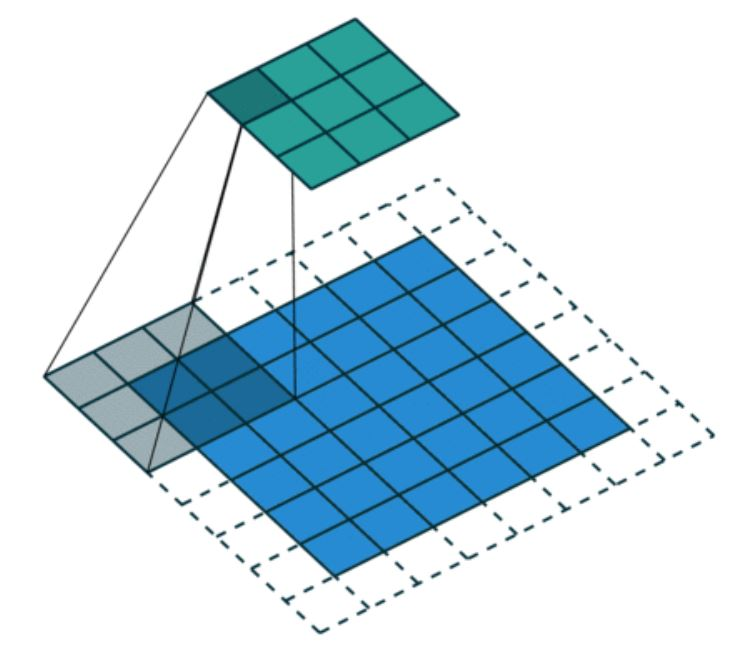
\includegraphics[width=7cm]{figure/chap4/CNN-op.jpg}
	  \bicaption[这里将出现在插图索引中]
		{卷积操作示意图}
		{A typical architecture of CNN}
	  \label{fig:chap4:cnn-op}
	\end{figure}
\subsection{池化层}
	池化层是一种对输入张量进行降采样的操作,由于其是在输入张量的每一个通道上进行的,所以不会改变通道的数目。
	池化操作可以大致分为最大值池化、均值池化和随机池化三种,
	其都是通过对输入张量一个邻域内的像素值进行聚合统计实现的。因为部分像素的改变并不会对聚合统计的结果
	造成太大的差异,因此池化操作具有一定的尺度不变性。如图\ref{fig:pooling}是三种池化操作的示意图,最大值
	池化求领域内特征点的最大值作为统计输出,均值池化求领域内特征点的平均值作为统计输出,随机池化将领域内
	特征点按照其数值大小赋予概率,然后按概率采样得到结果作为统计输出。
	\begin{figure}[h]
	  \centering
	  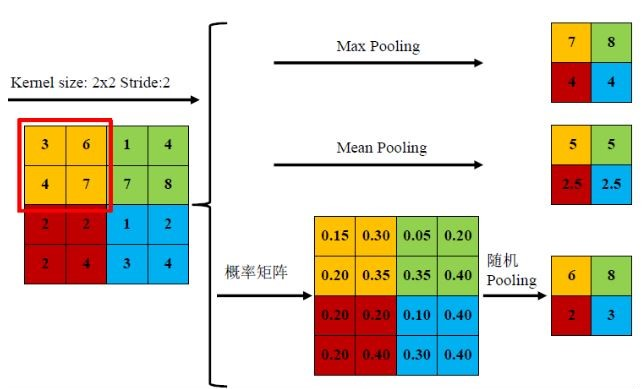
\includegraphics[width=8cm]{figure/chap4/pooling.jpg}
	  \bicaption[这里将出现在插图索引中]
		{卷积操作示意图}
		{A typical architecture of CNN}
	  \label{fig:pooling}
	\end{figure}
\subsection{Dropout层}
	为了解决神经网络过拟合的问题,Srivastava和Hinton等人\cite{srivastava2014dropout}于2014年提出dropout
	方法,有效的提高了网络的泛化能力。如图\ref{fig:dropout-connection}所示,在网络训练阶段,对每一个神经元以一定的概率
	丢弃。从而每次更新网络权值时,网络的连接都是随机的,相当于对采样到的网络进行更新。在网络测试阶段,为了
	得到所有随机连接网络的平均输出,这个阶段网络使用全连接的方式并且网络的权值以一定的比列缩放。
	\begin{figure}[!htp]    
\begin{minipage}[t]{0.5\linewidth}%设定图片下字的宽度,在此基础尽量满足图片的长宽    
	\centering    
	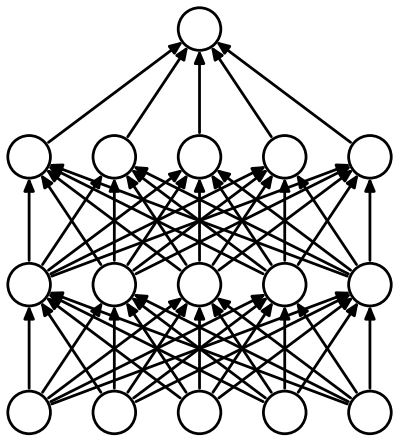
\includegraphics[width=0.9\linewidth]{figure/chap4/no-dropout.jpg}    
	\caption*{(a) 测试阶段网络连接 }
	\label{fig:no-dropout}    
\end{minipage}    
\begin{minipage}[t]{0.5\linewidth}%需要几张添加即可,注意设定合适的linewidth    
	\centering    
	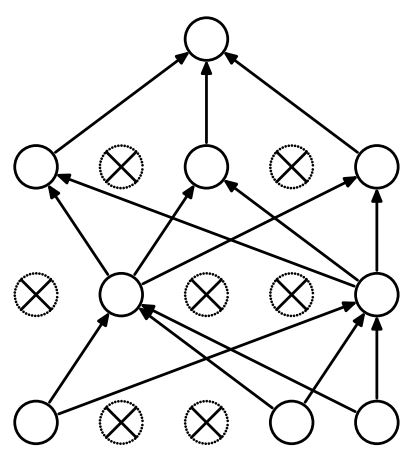
\includegraphics[width=0.9\linewidth]{figure/chap4/dropout.jpg}    
	\caption*{(b) 训练阶段网络的连接}
	\label{fig:dropout}
\end{minipage}
\bicaption{线虫弯曲角度和摆动频率的变换}{An EPS and PDF demo with subcaptionbox}%n张图片共享的说明
\label{fig:dropout-connection}
\end{figure}

\subsection{Batch Normalization层}
	批量标准化(Batch Normalization,BN)是深度学习领域一种非常重要的正则化的方法\cite{ioffe2015batch},有效的
	解决了内部方差偏移(Internal Covariate Shift)的问题。内部方差偏移指的是在网络训练的过程中,隐藏层的输入的
	分布一直在变,导致网络收敛变慢。批量标准化的方法可以使隐藏层的输入分布稳定并近似分从标准正态分布,很多
	激活函数(如tanh函数和sigmoid函数等)在0值附近的梯度是最大的,因此可以获得一个较大梯度,从而大大提高了网络的训练速度。
	另外,还降低了对初始学习率选取的敏感度。
\section{线虫轮廓解析方法介绍}
	本文提出的线虫轮廓解析方法的关键在于设计了一个只对位于图片中央的线虫轮廓敏感的神经网络,而对非图片中央位置的线虫轮廓不敏感。当输入
	一幅包含多线虫轮廓的前景图像时,网络的输出为中央线虫轮廓的图像。
	形式化的描述如下:假设一幅图片中包含N个线虫轮廓,定义一个集合$E =\{e_0,e_1,\dots,e_N\}$,其中$e_0$表示轮廓位于图片
	中央的线虫,$e_i$包含线虫重心坐标、轮廓以及方向等信息。$I(E)=R(\{e_0,e_1,\dots,e_N\};\xi)$表示由集合E渲染得到的包含N个线虫的图片,R表示
	渲染函数,$\xi$表示随机噪声。$I(E_0)=R(\{e_0\};\xi)$表示由中间线虫渲染得到的图片。我们希望得到这样的映射
	$S:I(E)\rightarrow I(E_0)$,映射函数$S$通过一个深度卷积网络加以实现,本文将其命名为SingleOut-net网络。
	\begin{figure}[htb]
	  \centering
	  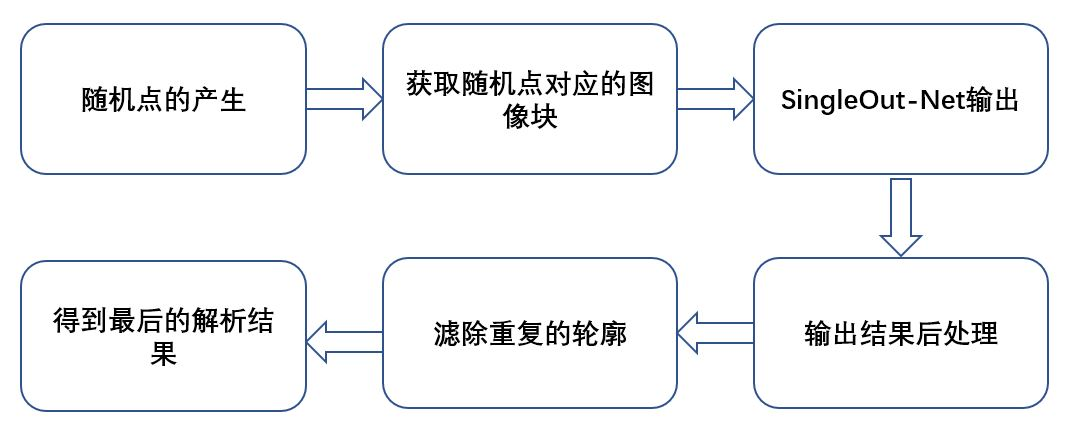
\includegraphics[width=9cm]{figure/chap4/flow.jpg}
	  \bicaption[这里将出现在插图索引中]
		{多线虫轮廓相互遮挡图片}
		{Change in contour curvature}
	  \label{fig:chap4:flow}
	\end{figure}
	
	如图\ref{fig:chap4:flow}是本文提出的线虫轮廓解析方法的主要流程。首先假定从前景提取的步骤中已经得到
	包含多线虫轮廓的二值化图像如图\ref{fig:multiworm}所示,在该二值化图像的前景像素中(即非零值像素)产生足够多的随机点使得每个线虫轮廓上至少
	包含一个随机点。然后以这些随机像素点为中心在原图中抠出固定尺寸的图像块,将这些图像块输入到训练好的SingleOut-Net
	网络从而得到中央线虫的轮廓。由于在随机点产生阶段,同一个线虫轮廓包含不止一个随机点。因此由SingleOut-Net网络输出
	的线虫轮廓包含同一个线虫的多个轮廓,在原图像坐标中,同一个线虫的多个轮廓是重合的。通过滤除掉重复的线虫轮廓以及
	不完整的轮廓,最终可以得到解析的结果。算法\ref{algo:worm_parser}描述线虫轮廓解析的整个算法实现。
\begin{algorithm}
\caption{线虫轮廓解析算法}
\label{algo:worm_parser}
\begin{algorithmic}[1]
\Require $Worm\_data$双重列表,$Worm\_data[i][j]$表示第$i$帧图像中第$j$只线虫。
\Ensure 输出$trackID$
  \algstore{MergeSort}
\end{algorithmic}
\end{algorithm}

\begin{algorithm}
\begin{algorithmic}[1]
  \algrestore{MergeSort}
\Function {Parser\_Worm}{$Worm\_Image$}
		\State $Seed\_points \gets Generate\_seed\_points(Worm\_Image)$
		\State $Image\_Patchs \gets Crop\_Image(Worm\_Image,Seed\_points)$
		\State $SingleOut\_OutputImages \gets []$
		\For{$i = 0 \to Image\_Patchs.length-1$}
			\State $SingleOut\_OutputImages[i] \gets SingleOut\_Net(Image\_Patchs[i])$
			\State $SingleOut\_OutputImages[i] \gets Post\_ProcessImage(SingleOut\_OutputImages[i])$
		\EndFor
		\State $Worm\_Contours \gets Extracte\_WormContour(SingleOut\_OutputImages)$
		\State $resulte \gets Filter\_WormContour(Worm\_Contours)$
		\State \Return $resulte$
\EndFunction
\end{algorithmic}
\end{algorithm}
		\begin{figure}[htp]
	  \centering
	  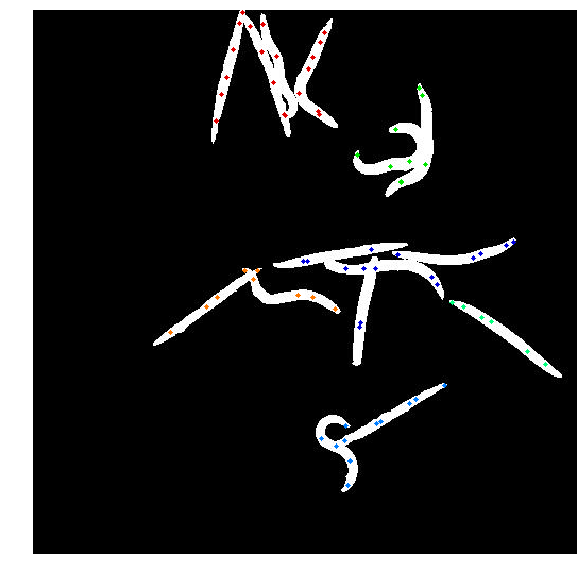
\includegraphics[width=9cm]{figure/chap4/rand_seed.png}
	  \bicaption[这里将出现在插图索引中]
		{多线虫轮廓相互遮挡图片}
		{Change in contour curvature}
	  \label{fig:chap4:rand_seed}
	\end{figure}
\subsection{随机点的产生}
	随机点的产生直接影响线虫轮廓解析方法的效率,随机点的数量过大导致SingleOut-Net网络需要对大量的图像块处理,需要很大
	的计算量,从而导致解析一帧图像需要大量的时间。但随机点的数量太少,可能导致有些线虫的轮廓上没有随机点,这些线虫的
	轮廓将得不到解析。实验发现,直接在原图像中生成随机点的方式非常的低效,主要是因为前景像素只占原图中总像素的一小部分。
	大部分的随机点落在了背景里。本文提出一种高效的随机点产生方法。首先,找出原图中所有的轮廓,然后在每个轮廓的边上等距
	的采样一定数量的边界点,最后在边界点的邻域内再采样。这种随机点产生的方法只需要产生少量的随机点即可覆盖所有的
	线虫轮廓,最终采样的结果如图\ref{fig:chap4:rand_seed}所示。

\subsection{SingleOut-Net网络输出后处理}
	图\ref{fig:chap4:singleout}显示了利用训练好的SingleOut-Net网络对部分图像块处理的结果。从图中可以看出SingleOut-Net
	网络成功的将位于图片中央的线虫轮廓从周围的线虫轮廓中分离出来。经过二值化等后处理步骤后,再用轮廓提取算法即可得到所有图像块
	对应的中央线虫的轮廓。
	但由于在随机点生成的过程中同一个线虫轮廓上可能包含
	多个随机点。所以在SingleOut-Net输出的结果中,同一个线虫的轮廓可能出现了多次。通过计算两个线虫轮廓在原图坐标中面积的
	重合度,当两个轮廓的重合度大于一个设定的阈值时,则只需保留其中的一个轮廓。当一个轮廓完全被另一个轮廓包含时,则保留
	轮廓面积较大的轮廓。过滤掉重复的轮廓以及不完整的轮廓后即可得到解析的结果,最终的解析结果如图\ref{fig:chap4:parser}
	所示。
	\begin{figure}[htb]
	  \centering
	  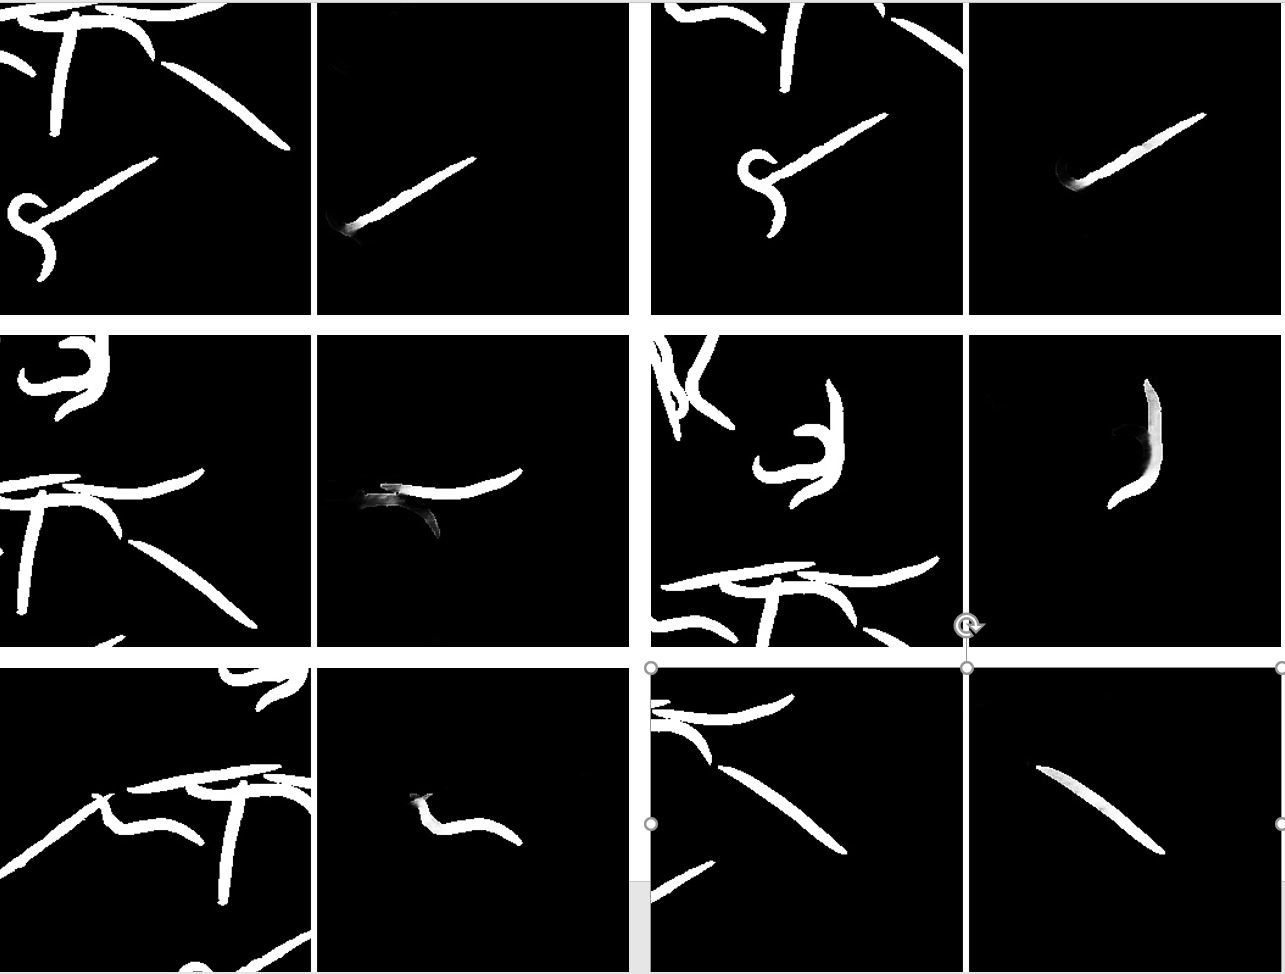
\includegraphics[width=8cm]{figure/chap4/singleout.jpg}
	  \bicaption[这里将出现在插图索引中]
		{多线虫轮廓相互遮挡图片}
		{Change in contour curvature}
	  \label{fig:chap4:singleout}
	\end{figure}
	\begin{figure}[htb]
	  \centering
	  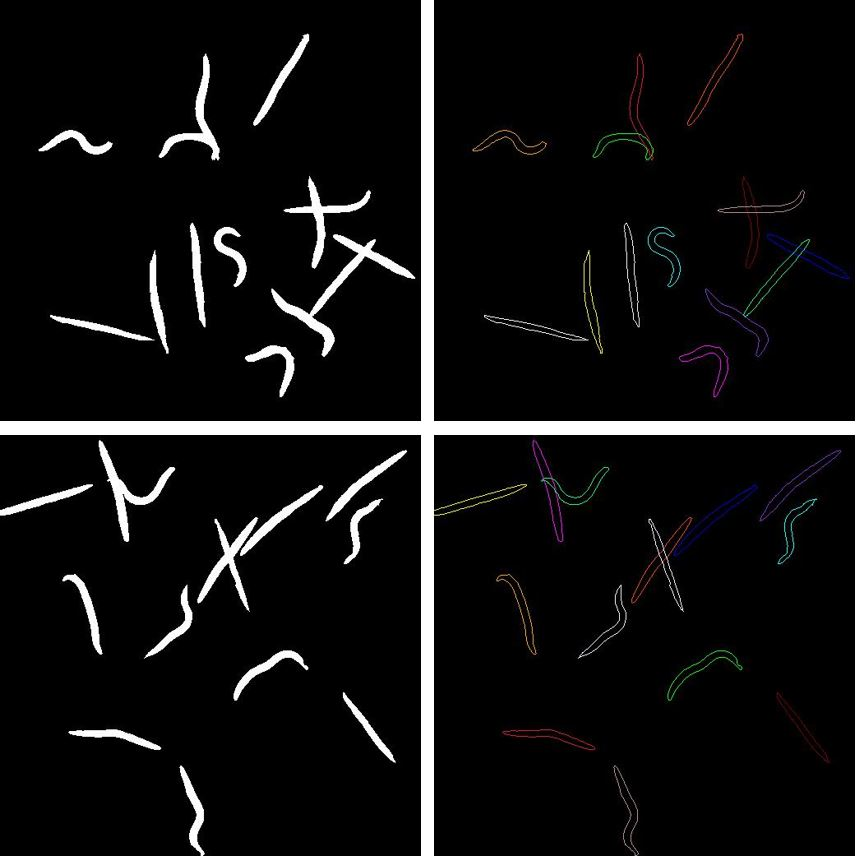
\includegraphics[width=7cm]{figure/chap4/Parser_Worms5.jpg}
	  \bicaption[这里将出现在插图索引中]
		{多线虫轮廓相互遮挡图片}
		{Change in contour curvature}
	  \label{fig:chap4:parser}
	\end{figure}
\section{SingleOut-net网络设计及模型评估}
	\begin{figure}[htb]
	  \centering
	  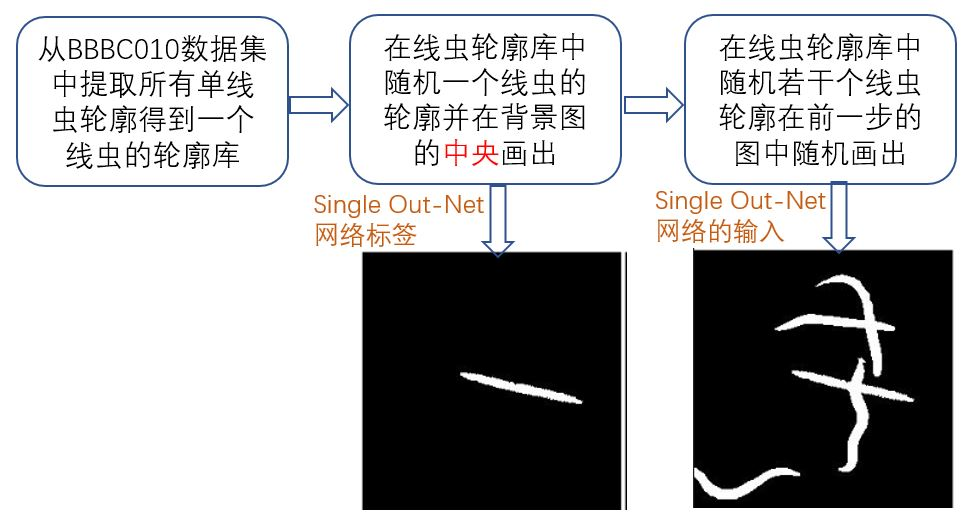
\includegraphics[width=11cm]{figure/chap4/dataset.jpg}
	  \bicaption[这里将出现在插图索引中]
		{多线虫轮廓相互遮挡图片}
		{Change in contour curvature}
	  \label{fig:chap4:dataset}
	\end{figure}
\subsection{训练集的制作}
\label{dataset}
	SingleOut-Net网络的训练需要大量的标定的数据集,本文采用了人工生成的数据集来训练网络的参数。
	数据集的制作流程如图\ref{fig:chap4:dataset}所示。
	BBBC010数据集\cite{Ljosa2012Annotated}中包含1407张单线虫轮廓的图像。首先,我们从BBBC010数据集中
	提取所有单线虫的轮廓得到一个单线虫的轮廓库。然后从单线虫的轮廓库中随机地选取一个线虫轮廓在一个
	分辨率为$256\times256$的背景图(像素值全为零)的中央画出。这一步得到的图作为网络训练的标签。继续从
	线虫轮廓库中随机选取若干个线虫的轮廓并在标签图像中随机的画出。至此,便得到了SingleOut网络的输入以及对应的
	标签。为了加快网络的收敛速度,本文将数据集的输入以及对应的输出归一化到$0\sim1$并加入一定量的高斯白噪声。
	通常数据集的多样性可以使神经网络学习到更多的模式,从而使网络具有更好的泛化能力。
	为了进一步增强数据集的多样性,本文对每个随机选取的单线虫轮廓进行随机的缩放和随机的旋转。

\subsection{网络结构的设计}
\label{archtecture}
\begin{figure}[htb]
	  \centering
	  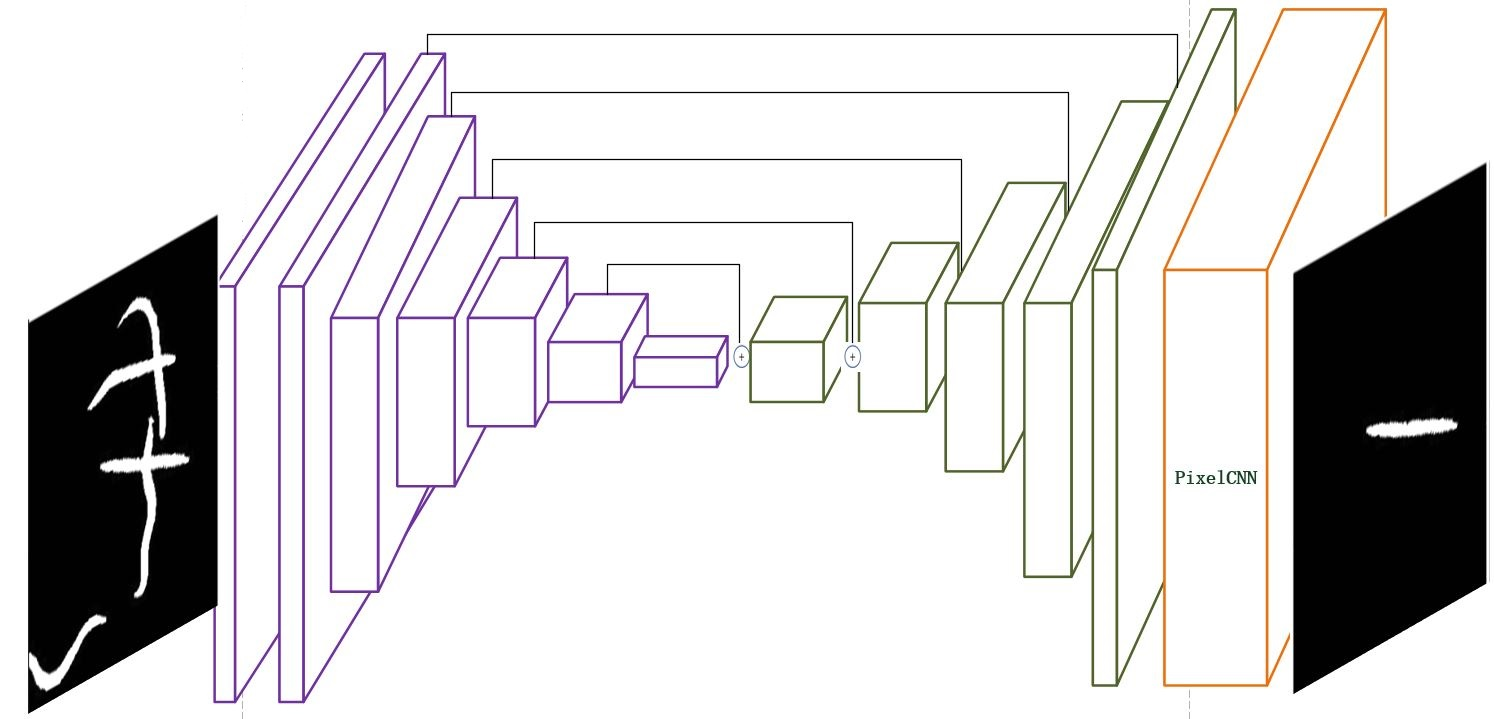
\includegraphics[width=14cm]{figure/chap4/arch1.jpg}
	  \bicaption[这里将出现在插图索引中]
		{多线虫轮廓相互遮挡图片}
		{Change in contour curvature}
	  \label{fig:chap4:netarch}
	\end{figure}
	如图\ref{fig:chap4:netarch}所示是SingleOut-Net的网络结构。输入为$256\times256\times1$的张量,输出也为
	相同尺寸的张量。整个网络架构由两个模块级联构成。第一个模块为一个类似于U-Net网络\cite{ronneberger2015u}的卷积模块在整个网络架构中
	相当于一个编码器,但与U-net网络使用的卷积模块不同,本文使用了如图\ref{fig:chap4:respool}所示的残差连接模块\cite{chu2017multi},这种残差
	模块包含三个连接通路。中间的通路由于使用了降采样,在卷积核尺寸保持不变的情况下,输出神经元的感受野将扩大到原来的两倍。
	但由于使用了降采样,所以导致分辨率下降。但上下两条路径上包含高分辨率的信息。最后将这三个路径的输出叠加在一起作为残差
	连接模块的输出。这种连接方式在扩大网络的感受野的同时依然保持原来的分辨率。第一个模块包含两条路径,分别为降采样路径和
	上采样路径。降采样路径上每经过一个残差连接模块后面都连接一个降采样层,将输入张量的尺寸减小一倍同时将通道数扩大一倍。
	降采样层通过一个卷积层实现,其卷积核的大小为$2\times2$步长为2。卷积后紧跟着的是Batch Normalization 层
	和激活函数层。由于Relu函数\cite{xu2015empirical}具有克服梯度消失和加快网络的收敛等优势,这里使用了Relu激活函数。
	在上采样路径与降采样路径类似,只不过将降采样层换成上采样层。上采样层通过反卷积实现,其卷积核大小为$2\times2$步长为2。
	如图\ref{fig:chap4:netarch}所示,上采样层的输入由两部分构成,分别为降采样路径中相同分别率的张量和上采样路径中前面的
	张量。第二个模块为一个PixelCNN网络\cite{van2016conditional}模块作为解码器。PixelCNN网络由Deepmind于2016年提出并用于
	条件图像生成。可以生成非常逼真的图像。本文将其应用在SingleOut网络中作为解码器来生成线虫图像。最后通过一个$1\times1$
	的卷积将通道数变为输出图像的通道数,并通过Sigmoid激活函数将输出的数值限制在$0\sim1$范围内。最终的输出是一个通道数为1
	的概率图。概率图中每一个像素值的大小表示该像素属于中央线虫轮廓的概率。
\begin{figure}[htb]
	  \centering
	  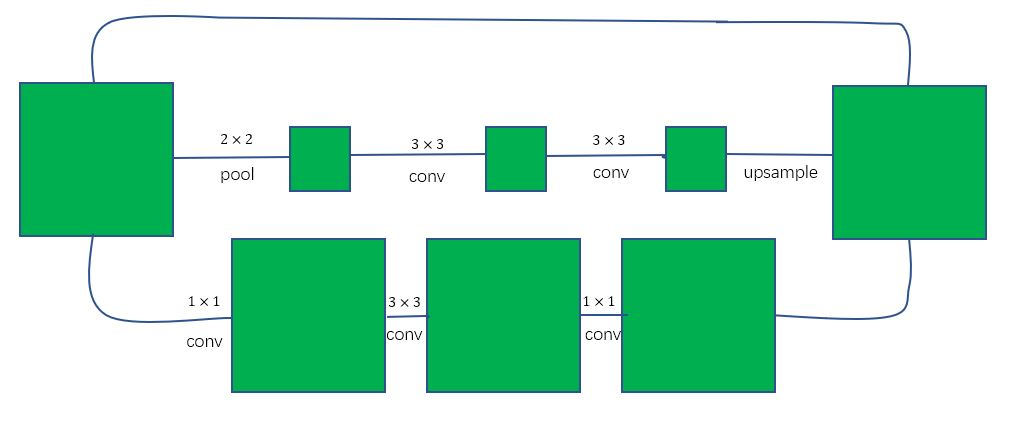
\includegraphics[width=9cm]{figure/chap4/residualpooling.jpg}
	  \bicaption[这里将出现在插图索引中]
		{多线虫轮廓相互遮挡图片}
		{Change in contour curvature}
	  \label{fig:chap4:respool}
	\end{figure}
\subsection{网络的训练及模型评价}
\subsubsection{损失函数}
	在对神经网络进行训练之前,首先需要确定网络训练的损失函数(也即目标函数)。神经网络通过不断地调整网络的
	模型参数使得训练损失不断减小。由上一小节可知,网络的最后一层输出是一张概率图设为$p$,$y$为标签图(只包含0和1)。
	公式\ref{eq:loss}表示网络训练的交叉熵损失。
	\begin{equation}
		entropy\_loss = \sum_{i,j}y_{ij}\log p_{ij} + (1-y_{ij})\log (1-p_{ij}) \label{eq:loss}
	\end{equation}
\subsubsection{评价指标}
	为了更好的对不同的网络架构进行量化分析和性能比较,因此需要选取一些评价指标。本文提出的SingleOut-Net网络
	用于判别图像中每个像素是否属于中央线虫轮廓像素,所以是一个像素二分类网络。本文将像素分类误差作为网络评价指标,
	像素分类误差由公式\ref{eq:metrics}表示。
	\begin{equation}
		pixel\_cls\_error =1- \frac{number\_of\_corrected\_classified\_pixels}{total\_number\_of\_pixels} \label{eq:metrics}
	\end{equation}
\subsubsection{网络的训练}
	
	根据\ref{dataset}节介绍的数据集生成方法,可以生成任意大小的训练集。但为了节省内存开销,本文采用了训练集动态生成的方法
	,即在训练阶段每个minibatch的样本图片都是动态生成的。但动态生成训练样本需要一定的时间开销,从而使网络训练时间变长。为了缩短网络训练时间以及在限定
	时间探索更优的网络架构,本文将数据生成和网络训练这两个任务并行,即用一个专门的线程负责数据集的生成。另外为了比较
	不同的网络架构的性能,测试集的样本应该保持不变,而本文中的数据集是动态随机生成的。为了获得一个不变的测试集,在网络训练和模型测试阶段,本文分别采用了
	两个不同的随机数种子初始化随机数生成器。
	
	在线虫的实时跟踪任务中,神经网络模型的复杂度和实时性是需要关注的重点。太复杂的网络其推断时间耗时太长往往达不到
	实时性的要求,因此必须要在网络结构的选取时加以考虑。而网络的训练和推断所消耗的时间的评估依赖于所采用的机器学习库
	和网络模型运行的硬件平台。因此为了评估不同网络模型的复杂度和实时性,表\ref{tab:hardwareconfig}
	列出了本文中所有网络模型运行的硬件平台。
	\begin{table}[!hpb]
	\centering
	\bicaption[指向一个表格的表目录索引]
    {算法运行的实验平台}
    {A Table}
	\label{tab:hardwareconfig}
	\begin{tabular}{p{80pt}p{100pt}}
	\toprule
	平台参数 & 配置 \\
	\midrule
	操作系统 & Windows 10 家庭版\\
	系统内存 & 8g \\
	CPU & i5-6300HQ \\
	GPU & GTX 950M \\
	显存 & 4g \\
	深度学习库 & Tensorflow \\
	\bottomrule
\end{tabular}
\end{table}
	
	神经网络模型的训练分为前向传播、反向传播和权值更新三个步骤。网络权值的更新往往是基于小批量样本而不是单个
	样本,其中batchsize是一个重要参数,其决定将多少样本作为一个整体估计梯度下降的方向。如果将其设置得过大,
	会导致网络模型陷入局部最小值点。如果设置得过小,则很难获得一个准确的梯度下降方向,在本文中batchsize的
	大小为4。神经网络的优化算法大致可以分为三大类:基于一阶微分的最优化方法(随机梯度下降)、基于二阶微分
	的最优化方法(牛顿法)以及基于二阶微分近似的方法(AdaDelta算法\cite{zeiler2012adadelta}和Adam算法\cite{kinga2015method}等)。随机梯度下降的最优化方法计算量
	最小,但网络的收敛速度慢。牛顿法由于利用了二阶信息,与其他的最优化方法相比具有更好的收敛性能,但由于要计算
	Hessian矩阵所以计算量很大。于是研究者们提出了很多基于二阶微分的近似方法,这些最优化方法是计算量和
	收敛性能的一个折中。本文采用了Adam最优化方法优化网络模型并将学习率设置为0.0002。训练40个epoch(每个epoch
	包含1000个batch)后网络已经完全收敛,图\ref{fig:chap4:loss}表示损失函数随epoch数的增加而下降。
	\begin{figure}[thb]
	  \centering
	  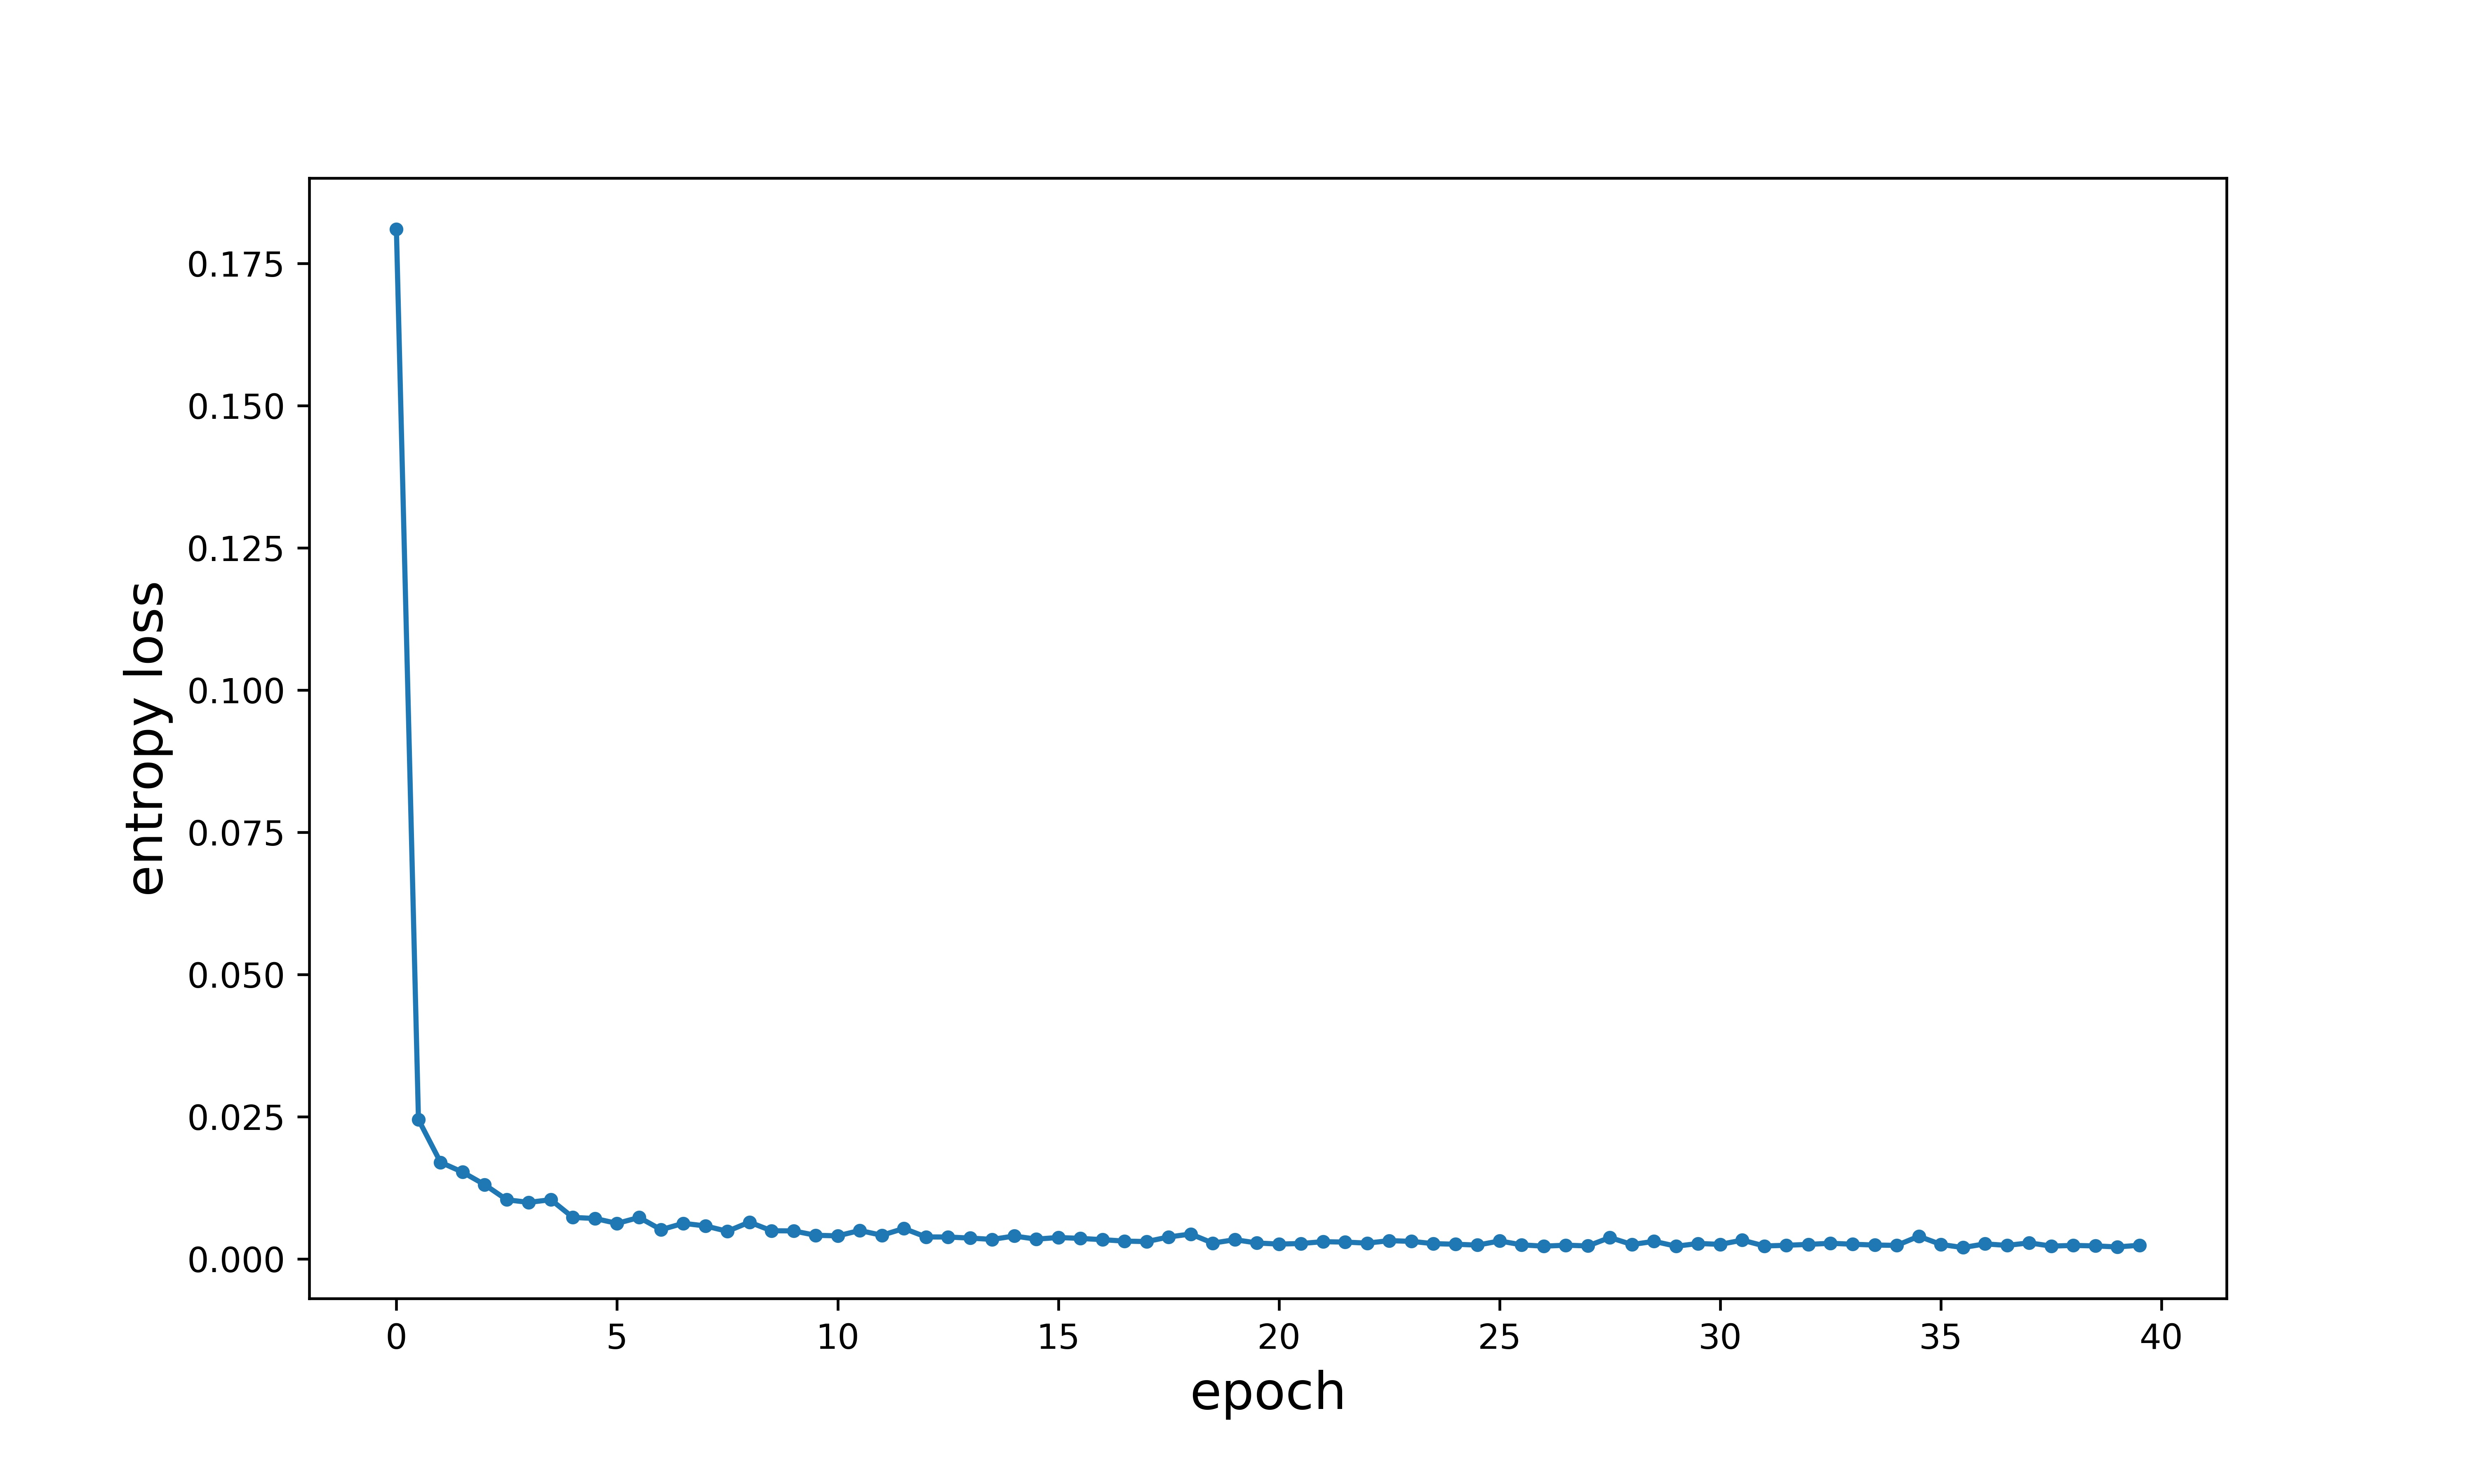
\includegraphics[width=13cm]{figure/chap4/loss.jpg}
	  \bicaption[这里将出现在插图索引中]
		{网络训练过程中损失函数的变化}
		{Change in contour curvature}
	  \label{fig:chap4:loss}
	\end{figure}
	
	为了观察网络训练过程中SingleOut-Net网络性能的变化,本文对网络每隔100次迭代进行一次测试,图\ref{fig:chap4:progress}
	显示了网络训练过程中对模型测试的结果。从图中可以看出随着网络模型迭代次数的增加SingleOut-Net网络逐渐学会过滤掉非中央
	线虫的轮廓,只保留中央线虫的轮廓。
		\begin{figure}[htb]
	  \centering
	  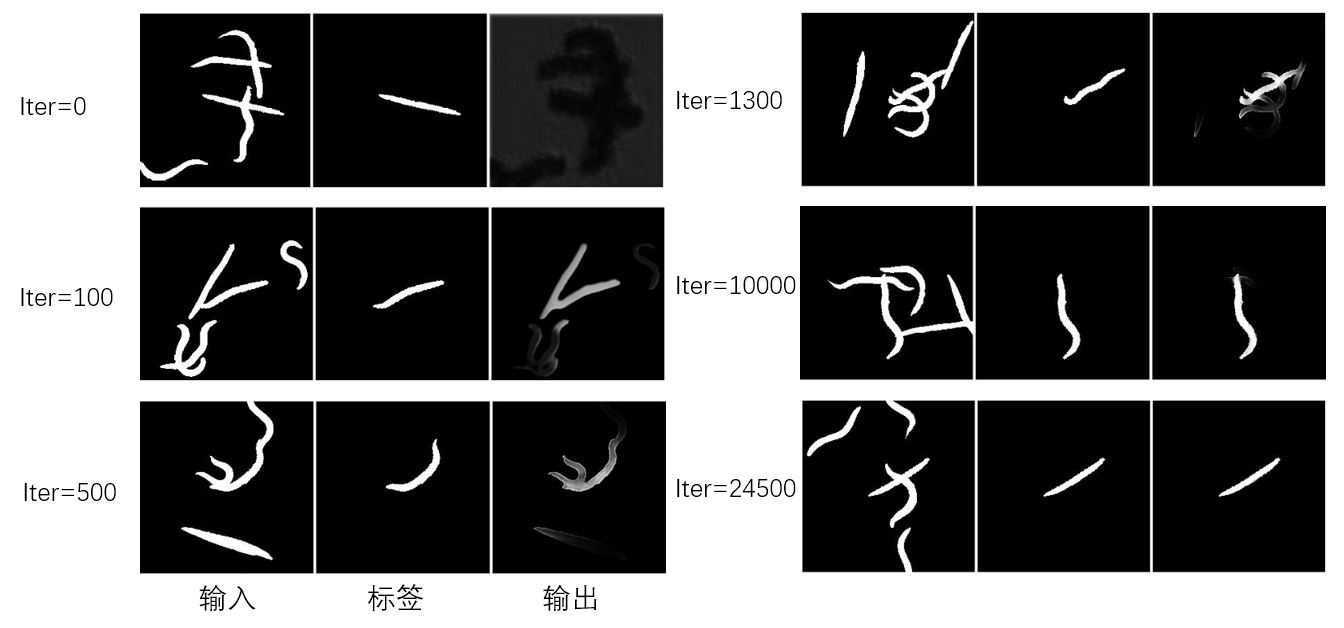
\includegraphics[width=13cm]{figure/chap4/progress.jpg}
	  \bicaption[这里将出现在插图索引中]
		{网络训练过程中模型测试结果}
		{Change in contour curvature}
	  \label{fig:chap4:progress}
	\end{figure}
\subsubsection{测试结果与分析}
	 在\ref{archtecture}节,本文介绍了SingleOut-Net的网络架构,由两个模块构成编解码器结构。后端模块是一个pixelCNN,
	 相当于一个解码器的作用。为了分析这种编解码结构的网络性能,本文分别从像素误差、模型复杂度和推断时间三个方面考察了
	 pixelCNN网络模块对整个网络架构的影响。由于pixelCNN网络模块的输入和输出的尺寸保持不变,所以可以将pixelCNN模块
	 移去,然后用一个$1\times1$的卷积将编码器输出的通道数变成网络最终输出的通道数。将这种没有pixelCNN模块的网络架构
	 命名为模型一,\ref{archtecture}节介绍的网络架构命名为模型二,两个模型的性能比较如表\ref{tab:performance}所示。
	 从表中可以看出pixelCNN网络模块可以显著的降低像素误差(10倍下降)。但同时由于增加了网络的深度,使得网络在推断单张图片所消耗
	 的时间变长,模型大小只有少量增加。
\begin{table}[!hpb]
	\centering
	\bicaption[指向一个表格的表目录索引]
    {网络模型性能的比较}
    {A Table}
	\label{tab:performance}
	\begin{tabular}{llll}
	\toprule
	网络模型 & 像素误差 & 模型大小 & 推断时间 \\
	\midrule
	模型一 &  0.00521\% & 46.8Mb & 31ms \\
	模型二 & 0.00045\% & 48.9Mb & 100ms \\
	\bottomrule
\end{tabular}
\end{table}
	 
\section{本章小结}
	
	


